\chapter{Linear function}
\section{Defined on $\mdr$}
\begin{theorem}[Solution formula for linear functions on $\mdr$]
    Let $f: \mdr \rightarrow \mdr $ be a linear function
    $f(x) := m \cdot x + t$ with $m \in \mdr \setminus \Set{0}$ and
    $t \in \mdr$ be a linear function.

    Then there is only one point $(x, f(x))$ on the graph of $f$ with
    minimal distance to $P = (x_P, y_P)$. This point is given by
    \[x = \frac{m}{m^2+1} \left ( y_P + \frac{1}{m} \cdot x_P - t \right )\]
\end{theorem}

\begin{figure}[htp]
    \centering
    \begin{tikzpicture}
        \begin{axis}[
            legend pos=north east,
            legend cell align=left,
            axis x line=middle,
            axis y line=middle,
            grid = major,
            width=0.8\linewidth,
            height=8cm,
            grid style={dashed, gray!30},
            xmin= 0, % start the diagram at this x-coordinate
            xmax= 5, % end   the diagram at this x-coordinate
            ymin= 0, % start the diagram at this y-coordinate
            ymax= 3, % end   the diagram at this y-coordinate
            axis background/.style={fill=white},
            xlabel=$x$,
            ylabel=$y$,
            tick align=outside,
            minor tick num=-3,
            enlargelimits=true,
            tension=0.08]
          \addplot[domain=-5:5, thick,samples=50, red] {0.5*x};
          \addplot[domain=-5:5, thick,samples=50, blue, dashed] {-2*x+6};
          \addplot[black, mark = *, nodes near coords=$P$,every node near coord/.style={anchor=225}] coordinates {(2, 2)};
          \newcommand{\R}{0.9}
          \addplot [domain=0:2*pi,samples=50, dotted]({\R*cos(deg(x))+2},{\R*sin(deg(x))+2});
          \addplot[blue, nodes near coords=$f_\bot$,every node near coord/.style={anchor=225}] coordinates {(1.5, 3)};
          \addplot[red, nodes near coords=$f$,every node near coord/.style={anchor=225}] coordinates {(0.9, 0.5)};
          \addlegendentry{$f(x)=\frac{1}{2}x$}
          \addlegendentry{$f_\bot(x)=-2x+6$}
        \end{axis}
    \end{tikzpicture}
    \caption{The shortest distance of $P$ to $f$ can be calculated by using the perpendicular}
    \label{fig:linear-min-distance}
\end{figure}

\begin{proof}
    With Theorem~\ref{thm:fermats-theorem} you get:
    \begin{align}
        0 &\stackrel{!}{=} (d_{P,f}(x)^2)'\\
        &= 2(x-x_P) + 2 (f(x) - y_P)f'(x)\\
        \Leftrightarrow 0 &\stackrel{!}{=} x - x_P + (f(x) - y_P) f'(x)\\
        &= x- x_P + (mx+t - y_P)\cdot m\\
        &= x (m+1) + m(t-y_P) - x_P\\
        \Leftrightarrow x &\stackrel{!}{=} \frac{x_p - m(t-y_p)}{m^2+1}\\
        &= \frac{m}{m^2+1} \left ( y_P + \frac{1}{m} \cdot x_P - t \right )\label{eq:solution-linear-r}
    \end{align}
    It is obvious that a minium has to exist, the $x$ from Equation~\ref{eq:solution-linear-r}
    has to be this minimum. $\qed$
\end{proof}
\clearpage

\section{Defined on a closed interval $[a,b] \subseteq \mdr$}
Let $f:[a,b] \rightarrow \mdr$, $f(x) := m\cdot x + t$ with $a,b,m,t \in \mdr$ and
$a \leq b$, $m \neq 0$  be a linear function.

\begin{figure}[htp]
    \centering
    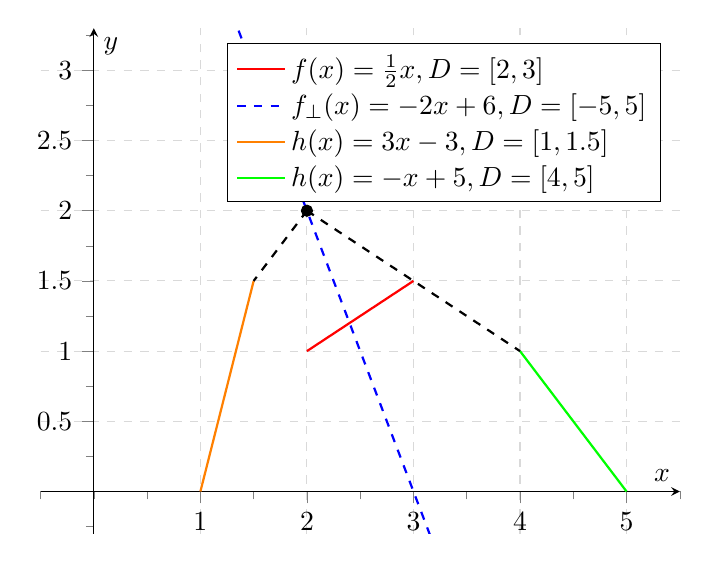
\begin{tikzpicture}
        \begin{axis}[
            legend pos=north east,
            legend cell align=left,
            axis x line=middle,
            axis y line=middle,
            grid = major,
            width=0.8\linewidth,
            height=8cm,
            grid style={dashed, gray!30},
            xmin= 0, % start the diagram at this x-coordinate
            xmax= 5, % end   the diagram at this x-coordinate
            ymin= 0, % start the diagram at this y-coordinate
            ymax= 3, % end   the diagram at this y-coordinate
            axis background/.style={fill=white},
            xlabel=$x$,
            ylabel=$y$,
            tick align=outside,
            minor tick num=-3,
            enlargelimits=true,
            tension=0.08]
          \addplot[domain= 2:3, thick,samples=50, red] {0.5*x};
          \addplot[domain=-5:5, thick,samples=50, blue, dashed] {-2*x+6};
          \addplot[domain=1:1.5, thick, samples=50, orange] {3*x-3};
          \addplot[domain=4:5, thick, samples=50, green] {-x+5};
          \addplot[black, mark = *, nodes near coords=$P$,every node near coord/.style={anchor=225}] coordinates {(2, 2)};
          \draw[thick, dashed] (axis cs:2,2) -- (axis cs:1.5,1.5);
          \draw[thick, dashed] (axis cs:2,2) -- (axis cs:4,1);
          \addlegendentry{$f(x)=\frac{1}{2}x, D = [2,3]$}
          \addlegendentry{$f_\bot(x)=-2x+6, D=[-5,5]$}
          \addlegendentry{$h(x)=3x-3, D=[1,1.5]$}
          \addlegendentry{$h(x)=-x+5, D=[4,5]$}
        \end{axis}
    \end{tikzpicture}
    \caption{Different situations when you have linear functions which
             are defined on a closed intervall}
    \label{fig:linear-min-distance-closed-intervall}
\end{figure}

The point with minimum distance can be found by:
\[\underset{x\in[a,b]}{\arg \min d_{P,f}(x)} = \begin{cases}
 S_1(f, P) &\text{if } S_1(f, P) \cap [a,b] \neq \emptyset\\
   \Set{a} &\text{if } S_1(f, P) \ni x < a\\
   \Set{b} &\text{if } S_1(f, P) \ni x > b
    \end{cases}\]

If $S_1(f, P) \cap [a,b] \neq \emptyset$, then $\underset{x\in[a,b]}{\arg \min d_{P,f}(x)} = S_1(f,P) \cap [a,b]$,
because $S_1(f,P)$ gives all global minima of $f$. Those are also
minima for the intervall $[a,b]$. There are not more minima, because
$S_1$ gives all minima of $P$ to $f$.

If $S_1(f, P) \cap [a,b] = \emptyset$, then it is not that simple.
But we can calculate the distance function:

\begin{align}
    d_{P,f}(x) &= \sqrt{(x-x_P)^2 + (f(x) - y_P)^2}\\
    &= \sqrt{(x^2 - 2x x_P + x_P^2) + (mx + (t-y_P))^2}\\
    &= \sqrt{(x^2 - 2x x_P + x_P^2) + m^2 x^2 + 2mx(t-y_P) + (t-y_P)^2}\\
    &= \sqrt{x^2(1+m^2) + x(-2 x_P + 2m(t-y_P)) + (x_P^2 + (t-y_P)^2)}
\end{align}

This function (defined on $\mdr$) is symmetry to the axis
\begin{align}
    x_S &= - \frac{-2 x_P + 2m(t-y_P)}{2(1+m^2)}\\
    &= \frac{x_P - m(t-y_P)}{1+m^2}\\
    &= \frac{m}{m^2+1} (y_P + \frac{1}{m} x_P - t)
\end{align}

$f$ is on $(-\infty, x_S]$ strictly monotonically decreasing and
on $[x_S, + \infty)$ strictly monotonically increasing.

Thus we can conclude:
\[\forall x,y \in \mdr: x \leq y < x_S \Rightarrow d_{P,f}(x_S) < d_{P,f}(y) \leq d_{P,f}(x)\]
\[\forall x,y \in \mdr: x_S < y \leq x \Rightarrow d_{P,f}(x_S) < d_{P,f}(y) \leq d_{P,f}(x)\]

When $S_1(f, P) \cap [a,b] = \emptyset$, then you can have two cases:
\begin{itemize}
    \item $a \leq b < x_S$: $b$ has the shortest distance in $[a,b]$
             on the graph of $f$ to $P$.
    \item $x_S < a \leq b$: $a$ has the shortest distance in $[a,b]$
             on the graph of $f$ to $P$.
\end{itemize}
